\section{Introduction}
\paragraph{\\\\Tree-depth definition\\\\}
In graph theory, the tree-depth is defined for undirected graphs. Intuitively, we may think of it as parameter that says how similar are G and a star, the lower tree-depth is the more "starlike" G is. Its value is between 1 and $|$G$|$. To explain the most common tree-depth definition, it is necessary to introduce term tree-depth decomposition. So tree-depth decomposition of graph G is a forest F with the following property:\\\\
\emph{If there is a edge uv in G then verticies u,v have ancestor-descendant relationship to each other in F.}\\\\
So the tree-depth of G is a depth of the forest with minimal depth among all tree-depth decomposition of G.\\\\
There is also recursive definition, that is worth to mention because of dynamic algorithm, that we are going to present in futher part of this documentation. The definition looks as follows:\\\\
\begin{equation}
td(G) =
\begin{cases}
1 & \text{if $|$G$|$=1}\\
1+min_{v \in V} td(G-v) & \text{if G is connected}\\
max_{i} td(G_{i})  & \text{otherwise}
\end{cases}       
\end{equation}
\\\\
\paragraph{Examples\\\\}
In this paragraph I will provide some obvious facts and examples of tree-depth decomposition in order to give reader a better intuition.\\\\
Only connected graph with tree-depth equal to 1 is \emph{K$_{1}$} and stars are only connected graphs with tree-depth equal to 2 and for these graphs graph and its best tree-depth decomposition is the same thing.\\\\
Antoher thing is that for every graph G a tree-depth depcomposition of G is a path P(where $|$P$|$=$|$G$|$) rooted in its beginning. It is true, because for such a tree every pair of vertices have ancestor-descendant relationship to each other.\\\\
The last fact, that I will point out is that if G is connected then its tree-depth decomposition F is also connected. It is true, because if F had two compositions, then there would be two groups of vertices in G without edges between each other, which is contradictiory to G being connected.
\begin{figure}[hbt!]
	\centering
	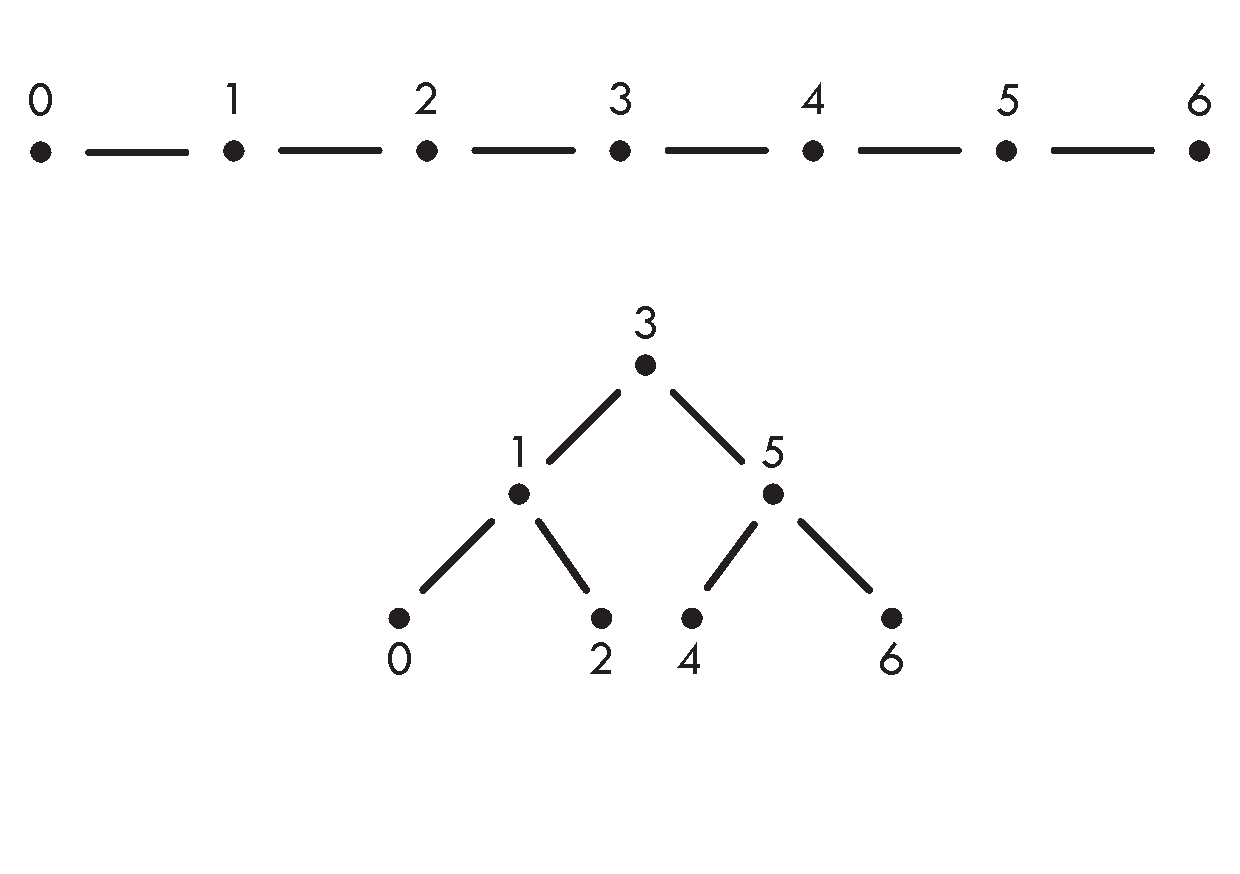
\includegraphics[scale=0.5,valign=t]{sciezka.pdf}
	\caption{P$_{7}$ and its tree-depth decomposition}
\end{figure}
\\\\\\\\
\begin{figure}[hbt!]
	\centering
	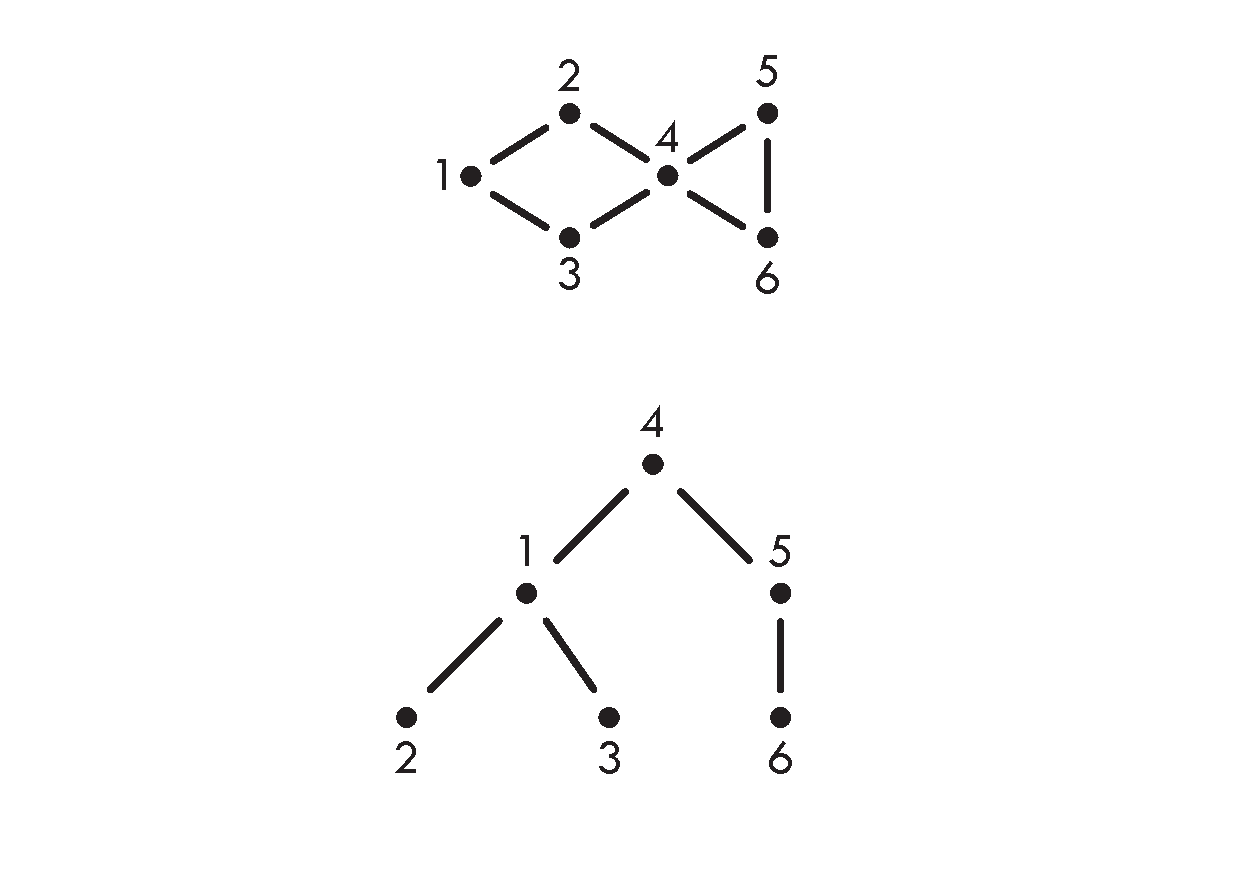
\includegraphics[scale=0.5,valign=t]{rybka.pdf}
	\caption{Fish and its tree-depth decomposition}
\end{figure}

